% Created by tikzDevice version 0.12.6 on 2026-07-03 04:21:18
% !TEX encoding = UTF-8 Unicode
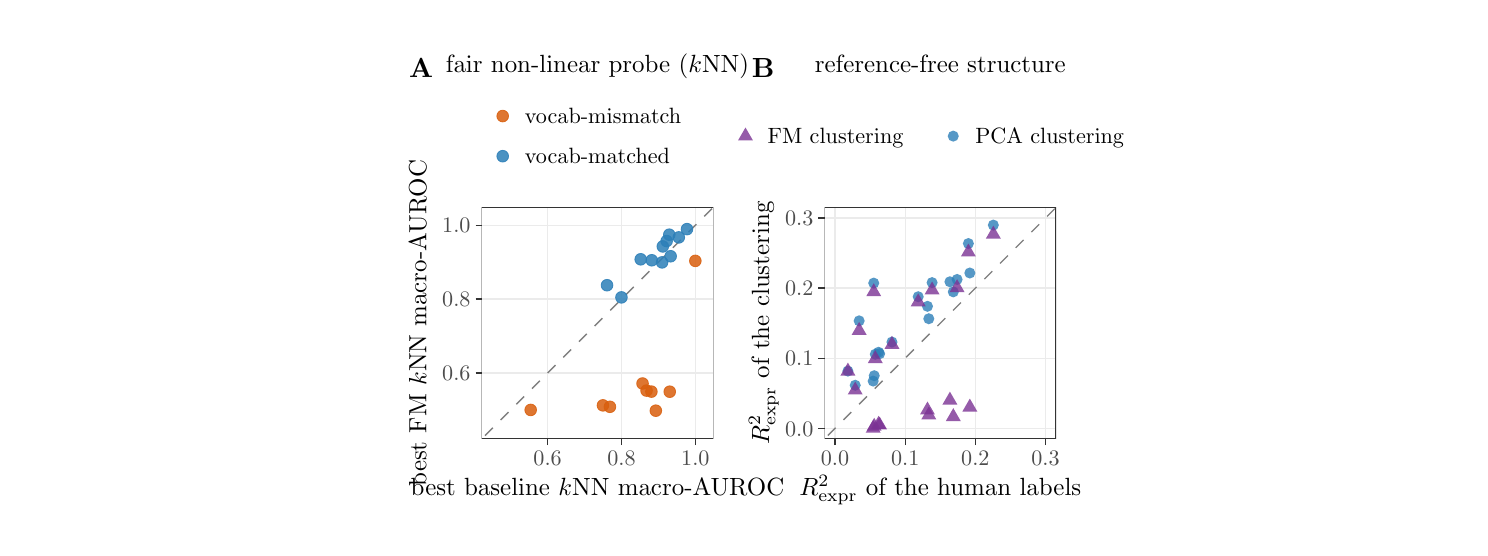
\begin{tikzpicture}[x=1pt,y=1pt]
\definecolor{fillColor}{RGB}{255,255,255}
\path[use as bounding box,fill=fillColor,fill opacity=0.00] (0,0) rectangle (517.45,180.67);
\begin{scope}
\path[clip] (127.85,  0.00) rectangle (389.61,180.67);
\definecolor{drawColor}{RGB}{255,255,255}
\definecolor{fillColor}{RGB}{255,255,255}

\path[draw=drawColor,line width= 0.5pt,line join=round,line cap=round,fill=fillColor] (127.85,  0.00) rectangle (389.61,180.67);
\end{scope}
\begin{scope}
\path[clip] (132.85,  5.00) rectangle (256.73,175.67);
\definecolor{drawColor}{RGB}{255,255,255}
\definecolor{fillColor}{RGB}{255,255,255}

\path[draw=drawColor,line width= 0.5pt,line join=round,line cap=round,fill=fillColor] (132.85,  5.00) rectangle (256.73,175.67);
\end{scope}
\begin{scope}
\path[clip] (256.73,  5.00) rectangle (380.61,175.67);
\definecolor{drawColor}{RGB}{255,255,255}
\definecolor{fillColor}{RGB}{255,255,255}

\path[draw=drawColor,line width= 0.5pt,line join=round,line cap=round,fill=fillColor] (256.73,  5.00) rectangle (380.61,175.67);
\end{scope}
\begin{scope}
\path[clip] (164.07, 32.07) rectangle (247.73,115.73);
\definecolor{fillColor}{RGB}{255,255,255}

\path[fill=fillColor] (164.07, 32.07) rectangle (247.73,115.73);
\definecolor{drawColor}{gray}{0.92}

\path[draw=drawColor,line width= 0.5pt,line join=round] (164.07, 55.88) --
	(247.73, 55.88);

\path[draw=drawColor,line width= 0.5pt,line join=round] (164.07, 82.57) --
	(247.73, 82.57);

\path[draw=drawColor,line width= 0.5pt,line join=round] (164.07,109.25) --
	(247.73,109.25);

\path[draw=drawColor,line width= 0.5pt,line join=round] (187.88, 32.07) --
	(187.88,115.73);

\path[draw=drawColor,line width= 0.5pt,line join=round] (214.57, 32.07) --
	(214.57,115.73);

\path[draw=drawColor,line width= 0.5pt,line join=round] (241.26, 32.07) --
	(241.26,115.73);
\definecolor{drawColor}{gray}{0.50}

\path[draw=drawColor,line width= 0.5pt,dash pattern=on 4pt off 4pt ,line join=round] ( 80.41,-51.59) -- (331.39,199.38);
\definecolor{drawColor}{RGB}{44,127,184}
\definecolor{fillColor}{RGB}{44,127,184}

\path[draw=drawColor,draw opacity=0.85,line width= 0.3pt,line join=round,line cap=round,fill=fillColor,fill opacity=0.85] (230.89,103.56) circle (  2.11);

\path[draw=drawColor,draw opacity=0.85,line width= 0.3pt,line join=round,line cap=round,fill=fillColor,fill opacity=0.85] (209.35, 87.60) circle (  2.11);
\definecolor{drawColor}{RGB}{217,95,14}
\definecolor{fillColor}{RGB}{217,95,14}

\path[draw=drawColor,draw opacity=0.85,line width= 0.3pt,line join=round,line cap=round,fill=fillColor,fill opacity=0.85] (225.38, 49.16) circle (  2.11);
\definecolor{drawColor}{RGB}{44,127,184}
\definecolor{fillColor}{RGB}{44,127,184}

\path[draw=drawColor,draw opacity=0.85,line width= 0.3pt,line join=round,line cap=round,fill=fillColor,fill opacity=0.85] (214.56, 83.21) circle (  2.11);

\path[draw=drawColor,draw opacity=0.85,line width= 0.3pt,line join=round,line cap=round,fill=fillColor,fill opacity=0.85] (225.52, 96.62) circle (  2.11);
\definecolor{drawColor}{RGB}{217,95,14}
\definecolor{fillColor}{RGB}{217,95,14}

\path[draw=drawColor,draw opacity=0.85,line width= 0.3pt,line join=round,line cap=round,fill=fillColor,fill opacity=0.85] (222.18, 52.09) circle (  2.11);
\definecolor{drawColor}{RGB}{44,127,184}
\definecolor{fillColor}{RGB}{44,127,184}

\path[draw=drawColor,draw opacity=0.85,line width= 0.3pt,line join=round,line cap=round,fill=fillColor,fill opacity=0.85] (229.25, 95.86) circle (  2.11);
\definecolor{drawColor}{RGB}{217,95,14}
\definecolor{fillColor}{RGB}{217,95,14}

\path[draw=drawColor,draw opacity=0.85,line width= 0.3pt,line join=round,line cap=round,fill=fillColor,fill opacity=0.85] (223.63, 49.53) circle (  2.11);
\definecolor{drawColor}{RGB}{44,127,184}
\definecolor{fillColor}{RGB}{44,127,184}

\path[draw=drawColor,draw opacity=0.85,line width= 0.3pt,line join=round,line cap=round,fill=fillColor,fill opacity=0.85] (232.34, 98.07) circle (  2.11);

\path[draw=drawColor,draw opacity=0.85,line width= 0.3pt,line join=round,line cap=round,fill=fillColor,fill opacity=0.85] (221.52, 96.97) circle (  2.11);

\path[draw=drawColor,draw opacity=0.85,line width= 0.3pt,line join=round,line cap=round,fill=fillColor,fill opacity=0.85] (235.28,104.89) circle (  2.11);

\path[draw=drawColor,draw opacity=0.85,line width= 0.3pt,line join=round,line cap=round,fill=fillColor,fill opacity=0.85] (229.50,101.62) circle (  2.11);
\definecolor{drawColor}{RGB}{217,95,14}
\definecolor{fillColor}{RGB}{217,95,14}

\path[draw=drawColor,draw opacity=0.85,line width= 0.3pt,line join=round,line cap=round,fill=fillColor,fill opacity=0.85] (241.26, 96.40) circle (  2.11);

\path[draw=drawColor,draw opacity=0.85,line width= 0.3pt,line join=round,line cap=round,fill=fillColor,fill opacity=0.85] (181.76, 42.54) circle (  2.11);

\path[draw=drawColor,draw opacity=0.85,line width= 0.3pt,line join=round,line cap=round,fill=fillColor,fill opacity=0.85] (226.98, 42.27) circle (  2.11);
\definecolor{drawColor}{RGB}{44,127,184}
\definecolor{fillColor}{RGB}{44,127,184}

\path[draw=drawColor,draw opacity=0.85,line width= 0.3pt,line join=round,line cap=round,fill=fillColor,fill opacity=0.85] (238.24,107.87) circle (  2.11);
\definecolor{drawColor}{RGB}{217,95,14}
\definecolor{fillColor}{RGB}{217,95,14}

\path[draw=drawColor,draw opacity=0.85,line width= 0.3pt,line join=round,line cap=round,fill=fillColor,fill opacity=0.85] (207.87, 44.19) circle (  2.11);
\definecolor{drawColor}{RGB}{44,127,184}
\definecolor{fillColor}{RGB}{44,127,184}

\path[draw=drawColor,draw opacity=0.85,line width= 0.3pt,line join=round,line cap=round,fill=fillColor,fill opacity=0.85] (231.84,105.86) circle (  2.11);
\definecolor{drawColor}{RGB}{217,95,14}
\definecolor{fillColor}{RGB}{217,95,14}

\path[draw=drawColor,draw opacity=0.85,line width= 0.3pt,line join=round,line cap=round,fill=fillColor,fill opacity=0.85] (232.01, 49.13) circle (  2.11);

\path[draw=drawColor,draw opacity=0.85,line width= 0.3pt,line join=round,line cap=round,fill=fillColor,fill opacity=0.85] (210.39, 43.67) circle (  2.11);
\definecolor{drawColor}{gray}{0.20}

\path[draw=drawColor,line width= 0.5pt,line join=round,line cap=round] (164.07, 32.07) rectangle (247.73,115.73);
\end{scope}
\begin{scope}
\path[clip] (  0.00,  0.00) rectangle (517.45,180.67);
\definecolor{drawColor}{gray}{0.30}

\node[text=drawColor,anchor=base east,inner sep=0pt, outer sep=0pt, scale=  0.80] at (160.02, 53.13) {0.6};

\node[text=drawColor,anchor=base east,inner sep=0pt, outer sep=0pt, scale=  0.80] at (160.02, 79.81) {0.8};

\node[text=drawColor,anchor=base east,inner sep=0pt, outer sep=0pt, scale=  0.80] at (160.02,106.50) {1.0};
\end{scope}
\begin{scope}
\path[clip] (  0.00,  0.00) rectangle (517.45,180.67);
\definecolor{drawColor}{gray}{0.20}

\path[draw=drawColor,line width= 0.5pt,line join=round] (161.82, 55.88) --
	(164.07, 55.88);

\path[draw=drawColor,line width= 0.5pt,line join=round] (161.82, 82.57) --
	(164.07, 82.57);

\path[draw=drawColor,line width= 0.5pt,line join=round] (161.82,109.25) --
	(164.07,109.25);
\end{scope}
\begin{scope}
\path[clip] (  0.00,  0.00) rectangle (517.45,180.67);
\definecolor{drawColor}{RGB}{0,0,0}

\node[text=drawColor,rotate= 90.00,anchor=base,inner sep=0pt, outer sep=0pt, scale=  0.90] at (144.05, 73.90) {best FM $k$NN macro-AUROC};
\end{scope}
\begin{scope}
\path[clip] (  0.00,  0.00) rectangle (517.45,180.67);
\definecolor{drawColor}{gray}{0.20}

\path[draw=drawColor,line width= 0.5pt,line join=round] (187.88, 29.82) --
	(187.88, 32.07);

\path[draw=drawColor,line width= 0.5pt,line join=round] (214.57, 29.82) --
	(214.57, 32.07);

\path[draw=drawColor,line width= 0.5pt,line join=round] (241.26, 29.82) --
	(241.26, 32.07);
\end{scope}
\begin{scope}
\path[clip] (  0.00,  0.00) rectangle (517.45,180.67);
\definecolor{drawColor}{gray}{0.30}

\node[text=drawColor,anchor=base,inner sep=0pt, outer sep=0pt, scale=  0.80] at (187.88, 22.51) {0.6};

\node[text=drawColor,anchor=base,inner sep=0pt, outer sep=0pt, scale=  0.80] at (214.57, 22.51) {0.8};

\node[text=drawColor,anchor=base,inner sep=0pt, outer sep=0pt, scale=  0.80] at (241.26, 22.51) {1.0};
\end{scope}
\begin{scope}
\path[clip] (  0.00,  0.00) rectangle (517.45,180.67);
\definecolor{drawColor}{RGB}{0,0,0}

\node[text=drawColor,anchor=base,inner sep=0pt, outer sep=0pt, scale=  0.90] at (205.90, 11.75) {best baseline $k$NN macro-AUROC};
\end{scope}
\begin{scope}
\path[clip] (  0.00,  0.00) rectangle (517.45,180.67);
\definecolor{fillColor}{RGB}{255,255,255}

\path[fill=fillColor] (162.15,124.73) rectangle (249.64,158.23);
\end{scope}
\begin{scope}
\path[clip] (  0.00,  0.00) rectangle (517.45,180.67);
\definecolor{fillColor}{RGB}{255,255,255}

\path[fill=fillColor] (166.65,143.73) rectangle (176.65,153.73);
\definecolor{drawColor}{RGB}{217,95,14}
\definecolor{fillColor}{RGB}{217,95,14}

\path[draw=drawColor,draw opacity=0.85,line width= 0.3pt,line join=round,line cap=round,fill=fillColor,fill opacity=0.85] (171.65,148.73) circle (  2.11);
\end{scope}
\begin{scope}
\path[clip] (  0.00,  0.00) rectangle (517.45,180.67);
\definecolor{fillColor}{RGB}{255,255,255}

\path[fill=fillColor] (166.65,129.23) rectangle (176.65,139.23);
\definecolor{drawColor}{RGB}{44,127,184}
\definecolor{fillColor}{RGB}{44,127,184}

\path[draw=drawColor,draw opacity=0.85,line width= 0.3pt,line join=round,line cap=round,fill=fillColor,fill opacity=0.85] (171.65,134.23) circle (  2.11);
\end{scope}
\begin{scope}
\path[clip] (  0.00,  0.00) rectangle (517.45,180.67);
\definecolor{drawColor}{RGB}{0,0,0}

\node[text=drawColor,anchor=base west,inner sep=0pt, outer sep=0pt, scale=  0.80] at (179.65,145.97) {vocab-mismatch};
\end{scope}
\begin{scope}
\path[clip] (  0.00,  0.00) rectangle (517.45,180.67);
\definecolor{drawColor}{RGB}{0,0,0}

\node[text=drawColor,anchor=base west,inner sep=0pt, outer sep=0pt, scale=  0.80] at (179.65,131.47) {vocab-matched};
\end{scope}
\begin{scope}
\path[clip] (  0.00,  0.00) rectangle (517.45,180.67);
\definecolor{drawColor}{RGB}{0,0,0}

\node[text=drawColor,anchor=base,inner sep=0pt, outer sep=0pt, scale=  0.90] at (205.90,164.48) {fair non-linear probe ($k$NN)};
\end{scope}
\begin{scope}
\path[clip] (  0.00,  0.00) rectangle (517.45,180.67);
\definecolor{drawColor}{RGB}{0,0,0}

\node[text=drawColor,anchor=base,inner sep=0pt, outer sep=0pt, scale=  1.00] at (142.19,162.71) {\bfseries A};
\end{scope}
\begin{scope}
\path[clip] (287.95, 32.07) rectangle (371.61,115.73);
\definecolor{fillColor}{RGB}{255,255,255}

\path[fill=fillColor] (287.95, 32.07) rectangle (371.61,115.73);
\definecolor{drawColor}{gray}{0.92}

\path[draw=drawColor,line width= 0.5pt,line join=round] (287.95, 35.87) --
	(371.61, 35.87);

\path[draw=drawColor,line width= 0.5pt,line join=round] (287.95, 61.22) --
	(371.61, 61.22);

\path[draw=drawColor,line width= 0.5pt,line join=round] (287.95, 86.57) --
	(371.61, 86.57);

\path[draw=drawColor,line width= 0.5pt,line join=round] (287.95,111.92) --
	(371.61,111.92);

\path[draw=drawColor,line width= 0.5pt,line join=round] (291.75, 32.07) --
	(291.75,115.73);

\path[draw=drawColor,line width= 0.5pt,line join=round] (317.10, 32.07) --
	(317.10,115.73);

\path[draw=drawColor,line width= 0.5pt,line join=round] (342.45, 32.07) --
	(342.45,115.73);

\path[draw=drawColor,line width= 0.5pt,line join=round] (367.80, 32.07) --
	(367.80,115.73);
\definecolor{drawColor}{gray}{0.50}

\path[draw=drawColor,line width= 0.5pt,dash pattern=on 4pt off 4pt ,line join=round] (204.29,-51.59) -- (455.27,199.38);
\definecolor{fillColor}{RGB}{44,127,184}

\path[fill=fillColor,fill opacity=0.80] (312.31, 67.08) circle (  2.00);

\path[fill=fillColor,fill opacity=0.80] (306.28, 62.67) circle (  2.00);

\path[fill=fillColor,fill opacity=0.80] (325.62, 75.49) circle (  2.00);

\path[fill=fillColor,fill opacity=0.80] (348.94,109.34) circle (  2.00);

\path[fill=fillColor,fill opacity=0.80] (299.03, 51.46) circle (  2.00);

\path[fill=fillColor,fill opacity=0.80] (333.25, 88.85) circle (  2.00);

\path[fill=fillColor,fill opacity=0.80] (321.79, 83.45) circle (  2.00);

\path[fill=fillColor,fill opacity=0.80] (340.45, 92.02) circle (  2.00);

\path[fill=fillColor,fill opacity=0.80] (305.72, 88.37) circle (  2.00);

\path[fill=fillColor,fill opacity=0.80] (296.39, 56.58) circle (  2.00);

\path[fill=fillColor,fill opacity=0.80] (339.92,102.67) circle (  2.00);

\path[fill=fillColor,fill opacity=0.80] (335.84, 89.69) circle (  2.00);

\path[fill=fillColor,fill opacity=0.80] (334.47, 85.20) circle (  2.00);

\path[fill=fillColor,fill opacity=0.80] (305.52, 52.96) circle (  2.00);

\path[fill=fillColor,fill opacity=0.80] (305.90, 54.91) circle (  2.00);

\path[fill=fillColor,fill opacity=0.80] (326.81, 88.55) circle (  2.00);

\path[fill=fillColor,fill opacity=0.80] (307.85, 62.84) circle (  2.00);

\path[fill=fillColor,fill opacity=0.80] (300.45, 74.73) circle (  2.00);

\path[fill=fillColor,fill opacity=0.80] (325.14, 79.98) circle (  2.00);

\path[fill=fillColor,fill opacity=0.80] (307.47, 63.38) circle (  2.00);
\definecolor{fillColor}{RGB}{123,50,148}

\path[fill=fillColor,fill opacity=0.80] (312.31, 69.31) --
	(315.01, 64.63) --
	(309.61, 64.63) --
	cycle;

\path[fill=fillColor,fill opacity=0.80] (306.28, 64.13) --
	(308.98, 59.46) --
	(303.58, 59.46) --
	cycle;

\path[fill=fillColor,fill opacity=0.80] (325.62, 43.80) --
	(328.32, 39.13) --
	(322.92, 39.13) --
	cycle;

\path[fill=fillColor,fill opacity=0.80] (348.94,109.13) --
	(351.64,104.46) --
	(346.24,104.46) --
	cycle;

\path[fill=fillColor,fill opacity=0.80] (299.03, 52.80) --
	(301.73, 48.13) --
	(296.33, 48.13) --
	cycle;

\path[fill=fillColor,fill opacity=0.80] (333.25, 49.15) --
	(335.95, 44.48) --
	(330.55, 44.48) --
	cycle;

\path[fill=fillColor,fill opacity=0.80] (321.79, 84.67) --
	(324.49, 79.99) --
	(319.09, 79.99) --
	cycle;

\path[fill=fillColor,fill opacity=0.80] (340.45, 46.64) --
	(343.15, 41.97) --
	(337.75, 41.97) --
	cycle;

\path[fill=fillColor,fill opacity=0.80] (305.72, 88.32) --
	(308.42, 83.64) --
	(303.02, 83.64) --
	cycle;

\path[fill=fillColor,fill opacity=0.80] (296.39, 59.65) --
	(299.09, 54.97) --
	(293.69, 54.97) --
	cycle;

\path[fill=fillColor,fill opacity=0.80] (339.92,102.67) --
	(342.62, 97.99) --
	(337.22, 97.99) --
	cycle;

\path[fill=fillColor,fill opacity=0.80] (335.84, 89.79) --
	(338.54, 85.11) --
	(333.14, 85.11) --
	cycle;

\path[fill=fillColor,fill opacity=0.80] (334.47, 43.19) --
	(337.17, 38.52) --
	(331.77, 38.52) --
	cycle;

\path[fill=fillColor,fill opacity=0.80] (305.52, 38.99) --
	(308.22, 34.31) --
	(302.82, 34.31) --
	cycle;

\path[fill=fillColor,fill opacity=0.80] (305.90, 39.70) --
	(308.60, 35.02) --
	(303.20, 35.02) --
	cycle;

\path[fill=fillColor,fill opacity=0.80] (326.81, 88.95) --
	(329.51, 84.28) --
	(324.11, 84.28) --
	cycle;

\path[fill=fillColor,fill opacity=0.80] (307.85, 40.15) --
	(310.55, 35.48) --
	(305.15, 35.48) --
	cycle;

\path[fill=fillColor,fill opacity=0.80] (300.45, 74.35) --
	(303.15, 69.68) --
	(297.75, 69.68) --
	cycle;

\path[fill=fillColor,fill opacity=0.80] (325.14, 45.58) --
	(327.84, 40.90) --
	(322.44, 40.90) --
	cycle;

\path[fill=fillColor,fill opacity=0.80] (307.47, 40.41) --
	(310.17, 35.73) --
	(304.77, 35.73) --
	cycle;
\definecolor{drawColor}{gray}{0.20}

\path[draw=drawColor,line width= 0.5pt,line join=round,line cap=round] (287.95, 32.07) rectangle (371.61,115.73);
\end{scope}
\begin{scope}
\path[clip] (  0.00,  0.00) rectangle (517.45,180.67);
\definecolor{drawColor}{gray}{0.30}

\node[text=drawColor,anchor=base east,inner sep=0pt, outer sep=0pt, scale=  0.80] at (283.90, 33.11) {0.0};

\node[text=drawColor,anchor=base east,inner sep=0pt, outer sep=0pt, scale=  0.80] at (283.90, 58.46) {0.1};

\node[text=drawColor,anchor=base east,inner sep=0pt, outer sep=0pt, scale=  0.80] at (283.90, 83.82) {0.2};

\node[text=drawColor,anchor=base east,inner sep=0pt, outer sep=0pt, scale=  0.80] at (283.90,109.17) {0.3};
\end{scope}
\begin{scope}
\path[clip] (  0.00,  0.00) rectangle (517.45,180.67);
\definecolor{drawColor}{gray}{0.20}

\path[draw=drawColor,line width= 0.5pt,line join=round] (285.70, 35.87) --
	(287.95, 35.87);

\path[draw=drawColor,line width= 0.5pt,line join=round] (285.70, 61.22) --
	(287.95, 61.22);

\path[draw=drawColor,line width= 0.5pt,line join=round] (285.70, 86.57) --
	(287.95, 86.57);

\path[draw=drawColor,line width= 0.5pt,line join=round] (285.70,111.92) --
	(287.95,111.92);
\end{scope}
\begin{scope}
\path[clip] (  0.00,  0.00) rectangle (517.45,180.67);
\definecolor{drawColor}{RGB}{0,0,0}

\node[text=drawColor,rotate= 90.00,anchor=base,inner sep=0pt, outer sep=0pt, scale=  0.90] at (267.93, 73.90) {$R^2_{\mathrm{expr}}$ of the clustering};
\end{scope}
\begin{scope}
\path[clip] (  0.00,  0.00) rectangle (517.45,180.67);
\definecolor{drawColor}{gray}{0.20}

\path[draw=drawColor,line width= 0.5pt,line join=round] (291.75, 29.82) --
	(291.75, 32.07);

\path[draw=drawColor,line width= 0.5pt,line join=round] (317.10, 29.82) --
	(317.10, 32.07);

\path[draw=drawColor,line width= 0.5pt,line join=round] (342.45, 29.82) --
	(342.45, 32.07);

\path[draw=drawColor,line width= 0.5pt,line join=round] (367.80, 29.82) --
	(367.80, 32.07);
\end{scope}
\begin{scope}
\path[clip] (  0.00,  0.00) rectangle (517.45,180.67);
\definecolor{drawColor}{gray}{0.30}

\node[text=drawColor,anchor=base,inner sep=0pt, outer sep=0pt, scale=  0.80] at (291.75, 22.51) {0.0};

\node[text=drawColor,anchor=base,inner sep=0pt, outer sep=0pt, scale=  0.80] at (317.10, 22.51) {0.1};

\node[text=drawColor,anchor=base,inner sep=0pt, outer sep=0pt, scale=  0.80] at (342.45, 22.51) {0.2};

\node[text=drawColor,anchor=base,inner sep=0pt, outer sep=0pt, scale=  0.80] at (367.80, 22.51) {0.3};
\end{scope}
\begin{scope}
\path[clip] (  0.00,  0.00) rectangle (517.45,180.67);
\definecolor{drawColor}{RGB}{0,0,0}

\node[text=drawColor,anchor=base,inner sep=0pt, outer sep=0pt, scale=  0.90] at (329.78, 11.75) {$R^2_{\mathrm{expr}}$ of the human labels};
\end{scope}
\begin{scope}
\path[clip] (  0.00,  0.00) rectangle (517.45,180.67);
\definecolor{fillColor}{RGB}{255,255,255}

\path[fill=fillColor] (249.88,131.98) rectangle (409.68,150.98);
\end{scope}
\begin{scope}
\path[clip] (  0.00,  0.00) rectangle (517.45,180.67);
\definecolor{fillColor}{RGB}{255,255,255}

\path[fill=fillColor] (254.38,136.48) rectangle (264.38,146.48);
\definecolor{fillColor}{RGB}{123,50,148}

\path[fill=fillColor,fill opacity=0.80] (259.38,144.59) --
	(262.08,139.92) --
	(256.68,139.92) --
	cycle;
\end{scope}
\begin{scope}
\path[clip] (  0.00,  0.00) rectangle (517.45,180.67);
\definecolor{fillColor}{RGB}{255,255,255}

\path[fill=fillColor] (329.45,136.48) rectangle (339.45,146.48);
\definecolor{fillColor}{RGB}{44,127,184}

\path[fill=fillColor,fill opacity=0.80] (334.45,141.48) circle (  2.00);
\end{scope}
\begin{scope}
\path[clip] (  0.00,  0.00) rectangle (517.45,180.67);
\definecolor{drawColor}{RGB}{0,0,0}

\node[text=drawColor,anchor=base west,inner sep=0pt, outer sep=0pt, scale=  0.80] at (267.38,138.72) {FM clustering};
\end{scope}
\begin{scope}
\path[clip] (  0.00,  0.00) rectangle (517.45,180.67);
\definecolor{drawColor}{RGB}{0,0,0}

\node[text=drawColor,anchor=base west,inner sep=0pt, outer sep=0pt, scale=  0.80] at (342.45,138.72) {PCA clustering};
\end{scope}
\begin{scope}
\path[clip] (  0.00,  0.00) rectangle (517.45,180.67);
\definecolor{drawColor}{RGB}{0,0,0}

\node[text=drawColor,anchor=base,inner sep=0pt, outer sep=0pt, scale=  0.90] at (329.78,164.48) {reference-free structure};
\end{scope}
\begin{scope}
\path[clip] (  0.00,  0.00) rectangle (517.45,180.67);
\definecolor{drawColor}{RGB}{0,0,0}

\node[text=drawColor,anchor=base,inner sep=0pt, outer sep=0pt, scale=  1.00] at (265.82,162.71) {\bfseries B};
\end{scope}
\end{tikzpicture}
